\chapter{Constrained optimisation}

In this chapter, we consider the problem
\[
\min_{x \in \mathcal{C}} f(x),
\]
where $\mathcal{C}$ is the feasible region\index{feasible!region}.
Usually, $\mathcal(C)$ is expressed as a collection of equalities and inequalities constraints:
\begin{align*}
  c_i(x) &\leq 0,\ i = 1,\ldots,m_1,\\
  c_i(x) &= 0,\ i = m_1+1,\ldots,m.
\end{align*}


\section{Projection methods}

We will restrict here to the case where the feasible region $C$ is a nonempty closed convex
subset of $\R^n$, on which projections are relatively easy to calculate.

\subsection{Bounds constraints}

One of the simplest feasible regions $\mathcal{C}$ is obtained when problem's variables
are subject to bounds constraints, i.e.
\[
 \mathcal{C} = \lbrace x_{\ell} \leq x \leq x_u \rbrace.
\]
The vectors $x_{\ell}$ and $x_u$ are the vectors of lower and upper bounds on the variables,
respectively, and we allow either of them to have components $-\infty$ of $+\infty$.

\begin{center}
\begin{minipage}{0.45\linewidth}
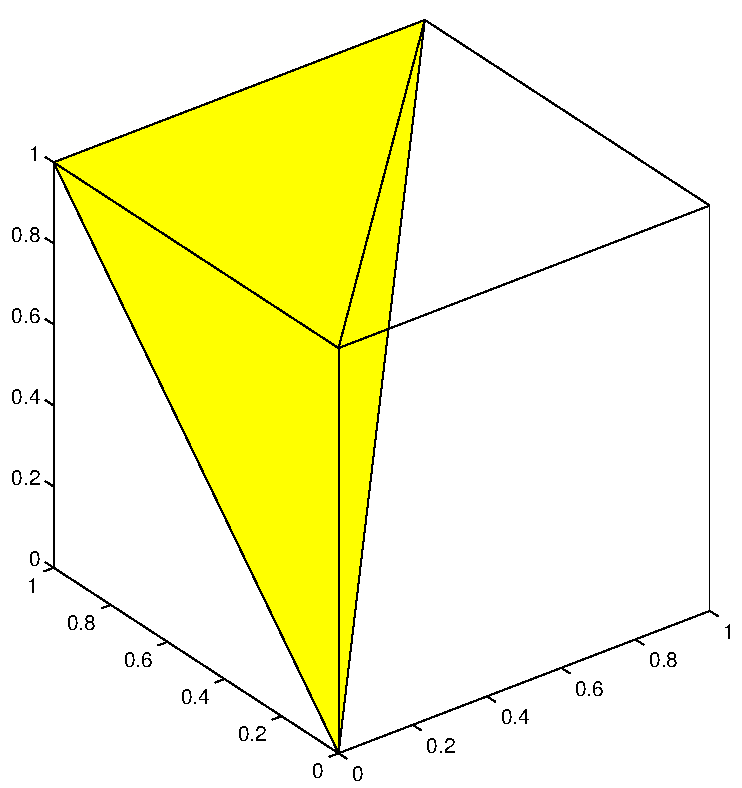
\includegraphics[width=0.9 \textwidth,clip]{osshape.pdf}\\
the order simplex in 3D
\end{minipage}
\begin{minipage}{0.45\linewidth}
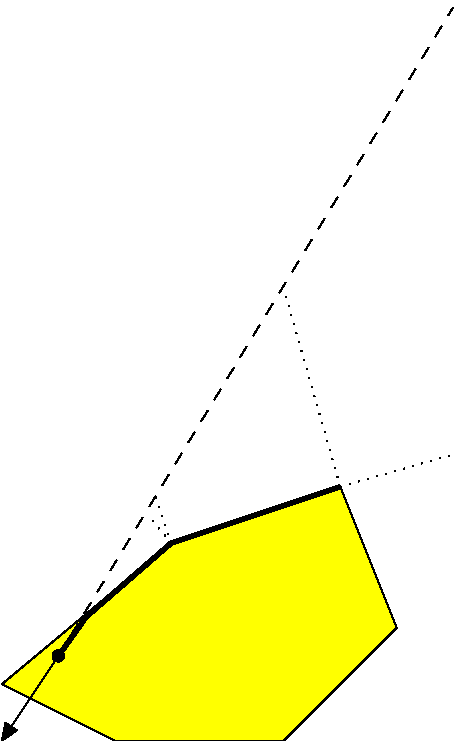
\includegraphics[width=0.9 \textwidth,height=0.9 \textwidth,clip]{pgpath.pdf}\\
the projected path
\end{minipage}
\end{center}
\section{Stopping criteria}

\subsection{Unconstrained optimisation}

Relative gradient. Dennis and Schnabel~\cite{DennSchn83}, Page 160.
\[
\max_i \frac{ \nabla f(x)_i \max \lbrace |x_i|, typ\ x_i\rbrace}
{\max \lbrace |f(x)|, typ\ f\rbrace},
\]
where $x_i$ is the $i^{th}$ component of the vector $x$.

\begin{verbatim}
double nlp_relative_gradient(double val, double *x, double *grad,
                             double *typx, int n, double typf)
\end{verbatim}

\subsection{Constrained optimisation}

\subsubsection{Projection methods for trust-region methods}

We use the criterion presented in Conn et al.~\cite{ConnGoulToin00},
Section~12.1:
\[
\| P[x-\nabla f(x)] - x \|_2 < \epsilon.
\]

\begin{verbatim}
int btr_constrained_projection_stopping_test(BTR *btr, double rho)
\end{verbatim}

\[
\max_i \frac{ \left(P[x-\nabla f(x)] - x\right)_i \max \lbrace |x_i|,
  typ\ x_i\rbrace} {\max \lbrace |f(x)|, f(typ\ f\rbrace},
\]
where $x_i$ is the $i^{th}$ component of the vector $x$.

\subsection{Specific projection algorithms}

\subsubsection{Isotonic regression}

Isotonic regression (IR) involves finding a weighted least-squares fit $x\in \R^n$ to a vector $a\in \R^n$ with weights vector $w\in \R^n$ subject to a set of monotonicity constraints giving a simple or partial order over the variables.
